\chapter{Principais trabalhos e \emph{datasets} estudados}

\section{Bitterlemons}
\label{bitter}

Falar de tudo e dos pre-processamentos

\chapter{Métodos baseados no emprego de palavras para identificação de perspectivas}
\label{chap3}

A classificação de um documento de acordo com sua perspectiva é o problema mais discutido nos artigos revisados para este projeto. Partindo da hipótese de que documentos escritos sob perspectivas diferentes costumam enfatizar termos distintos \cite{teubert}, classificadores podem ser empregados para, considerando apenas as diferentes ocorrências de palavras em documentos, identificar suas perspectivas. O número de ocorrências de uma palavra em um documento é comumente denominado de \textbf{contagem}; sendo assim, métodos baseados em \textbf{contagens de palavras} usam, como informação fundamental, o quanto elas ocorrem em documentos. De fato, grande parte dos artigos estudados para esta monografia classificam textos baseando-se em contagens de palavras, ainda que combinem, eventualmente, os resultados dos classificadores a outros métodos ou utilizem também outras características dos documentos. Pela relevância que a contagem de palavras tem na Mineração de Perspectiva, portanto, esse capítulo é totalmente dedicado à revisão e discussão de seu uso na identificação automática da perspectiva de documentos.
%ou mesmo utilizar palavras com conotações diferentes para um mesmo propósito,

Embora seja sempre possível associar contagens de palavras a aspectos temáticos, sintáticos e semânticos dos documentos, conduzindo a representações linguísticas mais complexas de cada um deles, este não é o enfoque dado pelos artigos revisados neste capítulo. Como será discutido nas próximas seções, a simples consideração das ocorrências de palavras em documentos costuma resultar em classificações de boa qualidade. Essa qualidade, entretanto, varia de acordo com o quanto essas ocorrências mudam de uma perspectiva para outra. Conforme observado na leitura dos artigos e em experimentos, quanto mais elas mudam, mais fácil se torna, para um classificador, aprender a perspectiva dos documentos.  %a diferença nas contagens de palavras  

Variações no uso de contagem de palavras foram encontradas em parte dos trabalhos estudados para este projeto: alguns deles utilizam valores \emph{booleanos} para indicar a presença (1) ou ausência (0) de palavras nos documentos, como o estudo de Klebanov, Beigman e Diermeier \cite{klebanov}, e outros empregam  as contagens normalizadas em relação ao corpus, como o trabalho de Hirst, Riabinin e Graham \cite{hirst-et-al}\footnote{Essas outras características aparecem ora combinadas entre si, ora associadas à contagem de palavras padrão, ora separadamente.}. De todo modo, a hipótese linguística assumida por eles, em suas metodologias, é a mesma: textos escritos sob perspectivas diferentes empregam palavras de forma distinta. \textbf{falar da figura}

% Decidiu-se discutir esses trabalhos também neste capítulo, pois

%, e há ainda aqueles que empregam a contagem de \textbf{sequências de palavras}, em vez de considerarem cada uma delas separadamente
%Em outras palavras, se as variações no uso de palavras são muito sutis, a tarefa de classificar documentos utilizando e % resultaificação de documentos de acordo com suas perspectivas. %pesar de simplificar bastante a estrutura dos documentos,  %Por se basearem apenas nas palavras dos documentos, portanto, os resultados desses artigos tendem a ser tão melhores quanto maior é a diferença no vocabulário de 

Este capítulo estrutura-se da seguinte forma: na seção \ref{freqs:revisao}, revisa-se artigos que utilizam contagens de palavras, ou variações, como elementos fundamentais de suas metodologias; na seção \ref{freqs:experim}, experimentos com um classificador Naïve Bayes e um modelo de tópicos L-LDA são conduzidos, a fim de se ilustrar as relações existentes entre o desempenho da classificação por perspectiva e o emprego de palavras nos documentos; por fim, a seção \ref{freqs:conc} apresenta considerações sobre as análises apresentadas nas seções \ref{freqs:revisao} e \ref{freqs:experim}. 





% a análise das relações existentes entre classificação baseada em contagens de palavras e a linguagem de diferentes perspectivas;

%Essa hipótese conduz à desconsideração de aspectos temáticos, sintáticos e semânticos dos documentos no momento de representá-los para a classificação. Por este motivo, como será discutido no decorrer deste capítulo,  



%Essa hipótese também implica na desconsideração do domínio temático dos documentos a serem classificados. Como será discutido no decorrer deste capítulo, a aplicação dessa hipótese conduz a resultados tão melhores quanto maior é a diferença no emprego de palavras por perspectiva. Isto significa que, em casos mais sutis, o descarte de aspectos temáticos, sintáticos e semânticos compromete significativamente a identificação da perspectiva de um documento. Ainda assim, muitos estudos relatam bons resultados considerando apenas essa hipótese - ou seja, baseando suas análises, basicamente, em contagens de palavras.


% o modo como palavras são empregadas  em um texto, desconsiderando-se quaisquer aspectos sintáticos ou semânticos, já evidencia pontos de vista distintos de forma suficiente.  %Isto reforça %Ainda assim, muitos estudos relatam bons resultados baseando-se apenas  

%uso de métodos baseados em contagseu uso.

%Neste capítulo, artigos que utilizam métodos baseados em frequências de palavras, e obtêm bons resultados, são revisados na seção \textbf{Trabalhos Analisados}. Experimentos conduzidos com um modelo de tópicos do tipo L-LDA\footnote{Este modelo de tópicos está descrito na seção \textbf{X} desta monografia.} e um classificador Naïve Bayes padrão\footnote{Este classificador está descrito na seção \textbf{X.X} desta monografia.}, apresentados na seção \textbf{Experimentos com L-LDA e Naïve Bayes}, ilustram a relação entre esse tipo de método e os vocabulários de diferentes perspectivas. Por fim, a seção \textbf{Conclusões} 


%Outro aspecto descartado por classificadores baseados 


% Os estudos apresentados neste capítulo, portanto, desconsideram tais aspectos
% FALAR DAS VARIAÇÕES: PRESENÇA, BIGRAMAS, TUDO JUNTO E MISTURADO. Variações encontradas em alguns trabalhos consistem em se utilizar os classificadores fixando-se, em vez de contagens de palavras, outras características dos


%Para os métodos revisados neste capítulo, a única informação extraída dos documentos é a frequência de suas palavras. Isto significa que a ordem das palavras em um documento, e as relações sintáticas que elas estabelecem entre si, não são consideradas. Os métodos também ignoram informações referentes ao domínio temático do \emph{dataset}. Apesar de simplificar bastante a estrutura linguística dos documentos, essa informação é a mais explorada pelos trabalhos estudados para esta monografia. Este capítulo revisa casos em que ela foi suficiente para, quando interpretada por um classificador, identificar as perspectivas de um corpus com boa taxa de acerto. 




% valores \emph{booleanos} que expressem suas presenças (1) ou ausências (0) no documento. % Trata-se, portanto, de classificar documentos a partir de suas representações como vetores, onde cada entrada corresponde a um número: a quantidade de vezes que certa palavra apareceu no texto (contagem) ou um \emph{booleano} que indique sua presença/ausência no mesmo. % baseada em documentos representados como vetores% explicitamente, %podem ser empregados para, aproveitando-se 


% Métodos baseados em frequências de palavras se apóiam na ideia de que é possível identificar a perspectiva de um documento analisando o seu vocabulário. Eles partem da hipótese de que documentos escritos sob perspectivas diferentes costumam dar destaque a termos distintos, mencionando-os com maior ou menor frequência a fim de reforçar ideias particulares \cite{teubert2001}. O emprego de palavras diferentes para um mesmo propósito, outra hipótese linguística assumida por métodos desse tipo, evidencia pontos de vista diferentes sobre um mesmo assunto. Um exemplo popular no Brasil é o uso dos termos \emph{Revolução} ou \emph{Golpe} para o mesmo evento histórico: o começo do Regime Militar Brasileiro. Enquanto o primeiro termo reflete a perspectiva pró-Ditadura, o segundo reflete a anti-Ditadura. Palavras como \emph{Revolução} e \emph{Golpe}, exploradas por diferentes perspectivas, são chamadas de \emph{banner words}, e têm o objetivo de facilitar a identificação entre adversários e aliados ideológicos \cite{teubert2001}.


%que indica que indivíduos defendendo perspectivas diferentes consolidam seus vocabulários através do uso de palavras específicas (\emph{stigma words} e \emph{banner words}), facilitando a identificação de adversários e aliados. 


%também evidencia perspectivas diferentes sobre um mesmo assunto e pode ser explorado por métodos desse tipo.



%diferencia documentos que tratam de um mesmo assunto é exemplo de como o vocabulário de um documento evidencia sua perspectiva sobre um determinado assunto.


\section{Trabalhos Revisados}
\label{freqs:revisao}

%Começar falando que os estudos têm em comum o uso de mét., em partic. NB e SVM, para a classificação de perspectivas de documentos. A forma como eles interp. e fazem uso desses resultados é o que mais profund. os diferencia. Essa seção discute como os artigos escolheram os métodos NB/SVM (1), mostra outros métodos, igualmente interessantes apesar de menos utilizados (2) e apresenta as discussões que eles trazem sobre as dificuldades e utilidades envolvidas na tarefa de classificação (3).

%Todos os trabalhos revisados para este projeto, que utilizam contagem de palavras e/ou alguma variação em suas metodologias, possuem pelo menos uma outra característica em comum: a classificação de documentos de acordo com suas perspectivas. O que varia de um para outro, além dos documentos \emph{per se}, são os classificadores e as discussões levantadas a partir dos resultados obtidos. Os classificadores mais utilizados nesses trabalhos foram Naïve Bayes e SVMs, mas dois artigos sugerem o uso de outros métodos: o trabalho de Lin et al., envolvendo documentos sobre o conflito Israel-Palestina, propõe o modelo LSPM a partir de uma modificação no Naïve Bayes \cite{lin-et-al2006}; e Laver, Benoit e College, por sua vez, apresentam o método Wordscores em um artigo no qual analisam posicionamentos de partidos políticos britânicos e irlandenses \cite{wordscores}. % As discussões levantadas nos estudos, por fim, tratam das dificuldades, aplicações e limitações envolvidas na classificação. %, suas aplicações e limitações. %Diante disso, esta seção revisa trabalhos 

Por questões de escopo, decidiu-se que, dentre os dez trabalhos revisados que tem diretamente a ver com este capítulo, apenas os dois mais citados  serão apresentados nesta seção\footnote{Os números de citações foram verificados no dia 22 de setembro de 2010, com auxílio do Google Scholar (http://scholar.google.com).}: o trabalho de Lin et al. \cite{lin-et-al2006}, envolvendo artigos sobre o conflito Israel-Palestina, e o primeiro artigo de Mullen e Malouf \cite{aaai-politics}, que analisa um fórum de discussão política dos Estados Unidos. Uma síntese dos outros oito encontra-se no \textbf{ANEXO BLI}, e informações referentes a eles são eventualmente mencionadas ao longo desta monografia.

%de Laver, Benoit e College \cite{wordscores},  no qual os autores analisam posicionamentos de partidos políticos britânicos e irlandenses;
\subsection{\emph{Which side are you on? Identifying perspectives at the document and sentence levels}}
\label{sec:lin-et-al}

O trabalho de Lin et al. analisa um conjunto de artigos sobre o conflito Israel-Palestina, escritos por especialistas no assunto e disponibilizados no \emph{site} Bitterlemons\footnote{http://www.bitterlemons.org/}. Os artigos, separados entre pró-Israel e pró-Palestina, são escritos por mais de 200 convidados e dois editores. Os autores realizam experimentos com classificadores Naïve Bayes e SVM para classificar os artigos de acordo com suas perspectivas, obtendo taxas de acerto mais altas com o Naïve Bayes (84.85\% a 93.46\% \emph{versus} 81.48\% a 88.22\%). O ponto mais importante deste artigo, entretanto, é a proposição do modelo generativo \emph{Latent Sentence Perspective Model} (\textbf{LSPM}), empregado também para classificação. % de modo semelhante ao Naïve Bayes.

%Este é um dos artigos mais citados pelos trabalhos revisados para esta monografia, e seu corpus já serviu como objeto de análise para outros estudos, incluindo este projeto. 
%Os autores realizam experimentos com um Naïve Bayes e um SVM, para classificação dos artigos de acordo com suas perspectivas. Nos dois casos, os artigos são representados como vetores - no primeiro, cada entrada corresponde à contagem de uma palavra; no segundo, essas contagens são normalizadas em relação ao resto do documento. O desempenho obtido com o Naïve Bayes foi melhor, e os autores sugerem que isso tem a ver com o tamanho do corpus: em tese, o Naïve Bayes precisa de menos documentos para treinamento, quando comparado com os SVMs, para atingir boa performance \cite{ng-jordan}. 

Diferentemente do Naïve Bayes, o LSPM associa uma variável latente a cada sentença de um documento, cujos valores indicam se ela carrega ou não a perspectiva do documento. O modelo, portanto, parte do pressuposto de que, até mesmo nos textos mais opinativos, é possível encontrar frases neutras que pouco colaboram para a identificação de sua perspectiva. No processo generativo, amostra-se uma classe para o documento; em seguida, para cada uma de suas sentenças, amostra-se um valor que indica se ela carrega (1) ou não (0) a perspectiva correspondente à classe; por fim, as palavras da sentença são geradas, baseando-se nessas duas informações (classe e presença de perspectiva).

O ponto chave do funcionamento desse modelo tem a ver com o fato de que todas as sentenças que não carregam uma perspectiva são tratadas da mesma forma: admite-se que elas poderiam ocorrer em qualquer documento, independentemente de sua classe. Isso faz com que as palavras geradas para essas sentenças sejam, na maioria das vezes, comuns em todo o corpus. As sentenças que carregam a perspectiva de seus documentos, por sua vez, tendem a gerar termos mais específicos, evidenciando as particularidades do vocabulário de cada ponto de vista. O modelo é adaptado para classificação de forma semelhante ao Naïve Bayes. A diferença principal é que, em vez de considerar o documento como um todo, apenas as palavras geradas por sentenças com perspectiva contribuem para a decisão de qual é a classe do documento. %considerando apenas as sentenças dos documentos de forma análoga ao Naïve Bayes.

%, independentemente da classe de seus documentos

No trabalho de Lin et al., a taxa de acerto obtida na classificação dos artigos com o LSPM foi ligeiramente superior àquela obtida com o Naïve Bayes -  86.99\% a 94.93\% \emph{versus} 84.85\% a 93.46\%. De todo modo, não foi encontrado nenhum outro artigo que faça uso do LSPM - provavelmente pelas dificuldades envolvidas em sua implementação, quando comparado ao Naïve Bayes. O tutorial de Resnik e Hardisty sobre Naïve Bayes e LSPM sugere algumas equações para a implementação dos modelos \cite{resnik}, mas o próprio Resnik afirmou, em \emph{e-mail} endereçado à autora desta monografia, nunca ter conseguido replicar os resultados apresentados por Lin et al.. Segundo ele, o modelo parece ser extremamente sensível ao valor dos hiperparâmetros escolhidos para as distribuições de probabilidade envolvidas \cite{mail-resnik}. Essas questões fazem do LSPM uma opção de classificador relativamente complexa. % como classificador.
% de modo que os termos mais específicos de cada perspectiva sejam gerados mais frequentemente em sentenças que a carregam

\subsection{\emph{A preliminary investigation into sentiment analysis of informal political discourse}}
\label{sec:aaai}

Esse trabalho de Mullen e Malouf analisa um conjunto de \emph{posts} do fórum Politics.com\footnote{http://politics.com}, escrito por cidadãos comuns dos Estados Unidos. Apesar de admitirem a diversidade de posicionamentos contidos no fórum, os autores dividem os documentos em apenas duas perspectivas, por uma questão de simplicidade: liberal e conservadora. Em seguida, eles condensam todos os \emph{posts} de um mesmo usuário em um só texto, resultando em um corpus com poucos documentos (96 liberais e 89 conservadores). Ao aplicar um Naïve Bayes para classificar os documentos de acordo com a orientação política de seus autores, a taxa de acerto obtida foi de 60.37\%. O tamanho do \emph{dataset} é apontado por Mullen e Malouf como um dos principais motivos para a obtenção desse resultado. De acordo com eles, a baixa taxa de acerto sugere que o Naïve Bayes é bastante sensível a uma pequena quantidade de artigos na etapa de treinamento. 

% Apesar disso, este trabalho contribui com algumas discussões interessantes sobre a linguagem dos \emph{posts} e as dificuldades envolvidas na tarefa de classificação.

Os autores discutem também outras hipóteses para o mau desempenho obtido na classificação desse corpus. Por ser composto de \emph{posts} de um fórum, por exemplo, a linguagem do corpus é bastante informal. A probabilidade de se encontrar uma mesma palavra escrita de várias formas é relativamente alta, o que pode criar um certo ruído na classificação dos documentos. Essa hipótese, entretanto, não foi comprovada pelos autores: em alguns experimentos com as palavras corrigidas, a taxa de acerto obtida com o Naïve Bayes foi ligeiramente mais alta (64.48\%); em outros, não (60.37\%). O artigo também sugere que a presença de documentos menores, correspondentes a usuários do fórum que raramente postam, pode contribuir negativamente para o desempenho do Naïve Bayes. A ideia é que, como esses usuários participam muito pouco do fórum, as palavras em seus \emph{posts} não são suficientes para se consolidar uma perspectiva, tornando-os mais difíceis de se classificar. Restringindo a classificação a usuários que postaram no fórum pelo menos 20 vezes, o número de documentos no corpus tornou-se ainda menor, mas a taxa de acerto obtida com o Naïve Bayes foi ligeiramente superior (61.38\%). 

Diante desses resultados, os autores sugerem que os usuários não estão se expressando de forma suficientemente diferente no nível das palavras, comprometendo o desempenho do Naïve Bayes. Uma última observação do artigo indica o que pode estar acontecendo: usuários liberais citam falas de usuários conservadores em 62.2\% de seus \emph{posts}; analogamente, conservadores citam liberais em 77.5\%  de seus \emph{posts}. Embora o artigo não indique a proporção média entre essas citações e o restante dos documentos, é possível que elas estejam interferindo negativamente no aprendizado das perspectivas. A presença das perspectivas liberal e conservadora em um mesmo documento, com uma correspondendo às intenções do usuário e outra sendo citada, pode homogeneizar o uso de palavras no corpus, comprometendo a viabilidade da classificação. Uma discussão interessante sobre esse tipo de problema é apresentada por Polanyi e Zaenen em seu artigo sobre aspectos linguísticos que interferem na análise de sentimento \cite{valence-shifters}.   




%do tempo; os conservadores, de forma análoga, citam os liberais Left users quote right users 62.2% do tempo e right quotes left 77.5% do tempo

%não há evidências suficientes de uma perspectiva em suas palavras



%são mais difíceis de se classificar. 

% - o que pode criar um ruído na classificação dos documentos. 


%, pois uma mesma palavra, dividida em várias \emph{versões} 



% do que em \emph{datasets}, compostos de artigos ou transcrições de debates. Esse fenômeno é tratado no artigo através da correção/padronização dessas palavras, evitando-se um ruído na classificação dos \emph{posts} \cite{aaai-politics}. 

%corpus de \emph{posts} do fórum Politics.com\footnote{http://politics.com}

%No caso do corpus \textbf{Bitterlemons}, dividido entre pró-Israel e pró-Palestina, há três tipos de sentença: neutra, que pode ocorrer em ambos os lados; pró-Israel, que carrega esta perspectiva; e pró-Palestina, análogo ao tipo pró-Israel. Sentenças pró-Israel ocorrem apenas em documentos classificados como pró-Israel, e o análogo vale para sentenças pró-Palestina. No processo generativo, o tipo neutro, por ocorrer em ambos os pontos de vista, passa a se associar às palavras mais comuns do corpus; palavras mais específicas de cada perspectiva são mais geradas por sentenças pró-Israel ou pró-Palestina. Neste sentido, o LSPM refina a noção de classe explorada pelo Naïve Bayes, admitindo a possibilidade de que determinadas palavras, por serem muito comuns, não adicionam informação relevante à classificação.



% pode ocorrer em ambos os lados, as palavras associadas a esses tipos de sentença vão assumindo as seguintes características: aquelas mais comuns em ambos os lados% Esses tipos de sentença  

%; no segundo, cada entrada corresponde simplesmente à contagem de uma palavra.
%As características dos documentos, consideradas na classificação,  são contagens de palavras e/ou suas variações, apresentadas na introdução deste capítulo.
%importantes obedecendo ao seguinte recorte:  

%\subsection{Os diferentes \emph{datasets}}

%Todos os \emph{datasets} revisados neste capítulo envolvem algum tema diretamente relacionado à política. A preferência por esse domínio temático provavelmente tem a ver com o fato de que, por ser polêmico, ele suscita a defesa clara de pontos de vista antagônicos, favorecendo a mineração de perspectivas. Os documentos são escritos por especialistas, jornalistas, pessoas políticas ou cidadãos comuns. As fontes também variam, envolvendo fóruns, transcrições de debates, \emph{blogs}, artigos e \emph{sites} especializados, o que colabora para a diversidade dos tipos de linguagem estudados. % defesas claras de pontos de vista antagônicos.


% Quando este não é o caso, tem-se um tema bastante polêmico, como pena de morte ou aborto. 


 %Em fóruns e \emph{blogs} mais informais, é preciso 

%O primeiro artigo de Mullen e Malouf revisado para esta monografia analisa um corpus de \emph{posts} do fórum Politics.com\footnote{http://politics.com}, escrito por cidadãos comuns dos Estados Unidos. Apesar de admitir a diversidade de posicionamentos contidos no fórum, os autores dividem os documentos em apenas duas perspectivas: liberal e conservadora. Por ser muito informal, a probabilidade de se encontrar palavras escritas de várias formas neste corpus é mais alta do que em outros, compostos de artigos ou transcrições de debates. Esse fenômeno é tratado no artigo através da correção/padronização dessas palavras, evitando-se um ruído na classificação dos \emph{posts} \cite{aaai-politics}. \textbf{Ver se bota nome después.}

%A linguagem dos fóruns muitas vezes se aproxima da linguagem falada, envolvendo gírias, expressões irônicas e certo nível de informalidade nas escolhas de palavras e construções sintáticas. Essas características também são encontradas em \emph{datasets} compostos de discursos políticos transcritos, por serem uma representação fiel de falas em discussões. A diferença fundamental entre textos recolhidos em fóruns e transcrições de debates políticos reside no fato de que os segundos apresentam menos erros gramaticais - e, portanto, menos necessidade de correção/padronização de palavras - do que os primeiros. 

%Três trabalhos que exploram debates políticos são revisados neste capítulo: os artigos de Laver, Benoit e College  \cite{wordscores}, envolvendo as políticas britânica e irlandesa; de Hirst, Riabinin e Graham, envolvendo a política canadense \cite{hirst-et-al}; e de Klebanov, Beigman e Diermeier, envolvendo a política dos Estados Unidos \cite{klebanov}. O primeiro analisa uma coleção \textbf{terminar}. O segundo analisa debates ocorridos em plenárias das \emph{English} e \emph{French House of Commons}, órgãos legislativos canadendes, durante os 36\textsuperscript{o}  e 39\textsuperscript{o} parlamentos. No 36\textsuperscript{o} parlamento, os liberais estavam no poder; no 39\textsuperscript{o}, os conservadores. O terceiro analisa debates sobre a legalização do aborto, desenvolvidos na \emph{House of Representatives}, órgão similar à Câmara Federal dos Deputados brasileira, e no Senado dos Estados Unidos. Os debates ocorreram entre os anos de 1995 e 2003, e estão divididos entre pró-escolha e pró-vida. %, órgão próximo    %próximos à Câmara 

%Com conteúdo extraído de mais de 250 \emph{blogs}, o artigo de Durant e Smith explora textos que discutem os posicionamentos de George W. Bush perante a Guerra do Iraque. Os \emph{posts} pertencem a \emph{blogs} de especialistas e cidadãos comuns, listados no \emph{site} The Moderate Voice\footnote{http://themoderatevoice.com/} e separados entre esquerda e direita. O périodo analisado se estendeu de março de 2003 a março de 2005. Baseando-se no fato de que o uso de palavras muda significativamente em um período de dois anos, conforme novos acontecimentos vão sendo discutidos nos \emph{blogs}, Durant e Smith particionaram seu corpus em 25 segmentos, cada um correspondendo ao conteúdo de um mês. Essa estratégia valorizou os acontecimentos políticos particulares de cada mês, que se refletem diretamente na ênfase, dada pelos blogueiros, a determinadas palavras.


%Ainda em política:  blog (listas), coluna (bitterlemons) e notícia (métrica).
%Ainda em política, o trabalho de Lin et al. analisa um conjunto de artigos sobre o conflito Israel-Palestina, escritos por especialistas no assunto e disponibilizados no \emph{site} Bitterlemons.com\footnote{http://www.bitterlemons.org/}. Os artigos, separados entre pró-Israel e pró-Palestina, são escritos por mais de 200 convidados e dois editores. Este é um dos artigos mais citados pelos trabalhos revisados para esta monografia, e o corpus por ele avaliado também já serviu como objeto de análise para outros estudos, incluindo esta monografia. O artigo de Klebanov, Beigman e Diermeier, por exemplo, também apresenta um estudo envolvendo todos os artigos desse corpus escritos por convidados \cite{klebanov}. Esse mesmo artigo, por fim, também explora o conteúdo de \emph{sites} especializados na questão da pena de morte nos Estados Unidos. O corpus, criado por Stephen Greene para sua tese de doutorado, é composto de cinco \emph{sites} pró-pena e três anti-pena \cite{greene-thesis}. %Nem a tese nem o artigo de Klebanov, Beigman e Diermeier informam 

%Klebanov, Beigman e Diermeier também analisam \emph{datasets} com outras temáticas, como legalização do aborto e pena de morte.

% Apesar de não haver um grande compromisso entre os \emph{posts} e a correção gramatical, os autores não relatam nenhum tratamento a erros gramaticais contidos nos textos, relativamente informais. % correspondentes a cada mês, valorizando diferentes destaques a termos



% cada um deles contendo todos os \emph{posts} escritos em um mês.

  % We chose to partition our slightly greater than two years of data by the month; thus
%creating twenty-five partitions. We predict the sentiment of political web posts for
%each of the 25 different time segments. We believe our data and many of our terms to
%be time-specific so we keep our data time-ordered. We chose our time interval to be a
%month because we needed an interval large enough to ensure enough postings to cre-
%ate good-sized datasets yet small enough to limit the number of events discussed
%within the interval.





%We used both the English and French House of Commons Debates (“Hansard”) for the first
%350 sitting days of the 36th Parliament (1997-09-22 to 2000-05-10). In the 36th Parliament,
%a majority government was formed by the Liberal Party, led by Jean Chrétien. This data was
%available in a convenient plain-text form with sentence breaks identified (Germann, 2001), as it
%has been widely used for research in machine translation.



%temas polêmicos 

%Para métodos que classificam documentos baseando-se em contagens de palavras ou variações, esse fenômeno pode gerar um ruído indesejado, pois os classificadores atribuirão contagens distintas a \emph{versões} de uma mesma palavra.

%, que analisa as perspectivas contidas no fórum de discussão política Politics.com\footnote{http://politics.com},




%Cada tipo de fonte sustenta determinadas características, que precisam ser devidamente investigadas antes da classificação dos documentos. 

%Em fóruns e \emph{blogs} mais informais, por exemplo,   O primeiro artigo de Mullen e Malouf, que analisa as perspectivas contidas no fórum de discussão política Politics.com\footnote{http://politics.com}, sugere que, nestes casos, seja feita uma correção das palavras antes da etapa de classificação \cite{aaai-politics}.  %interpretarão como duas palavras diferentes - com contagens diferentes. o que pode exigir correções 




%Quão mais informal é a fonte, por exemplo, maior é a probabilidade de se encontrar palavras escritas incorretamente. % palavras escritas maior é a probabilidade de conter uma quantidade significativa de palavras escritas incorretamente, o   
%predileção por datasets políticos. falar das fonotes diferentes, e de como isso tem certo impacto no pré-processamento e no que se espera da classificação.

%\subsection{Os diferentes classificadores}

%predileção por svms/naive bayes. falar oq cada lado defende. indicar q isso é bobo. apresentar lspm e wordscores.

%\subsection{As diferentes características dos documentos consideradas}

%falar das características usadas, em separado ou em combinado, e as discussões sobre qtas usar e quais usar.

%\subsection{As diferentes discussões}

%Várias coisas. De bias em jornais até estar ou n classificando estilo até a consolidação de uma perspectiva até internacionalização até etc.






%  perspectivas de partidos Britânicos sobre a política econômica do Reino Unido.

%ESTIMATING THE POLICY POSITIONS OF BRITISH AND IRISH PARTIES ON THE
 %        LIBERAL-CONSERVATIVE SOCIAL POLICY DIMENSION

%British party positions on economic policy
%utilizam e %são consideradas 

%Um certo padrão emerge dos estudos: uma preferência por corpora políticos (e falar aí de como eles usam diferentes fontes e aplicam o resultado da classificação para análises diferentes.
%e por classificadores Naïve Bayes e SVM. 
%Há casos em que o SVM se sai melhor e há casos em que o Naive Bayes se sai melhor. Argumentar a favor de escolher arbitrariamente e, se insatisfeito com o desempenho, testar outro, pq é isso que algumas pessoas fazem.
%Discutir as características escolhidas e a redução de features
%Discutir a classificação efetiva de pontos de vista, n estilos. 

%descritos na seção \textbf{Experimentos com L-LDA e Naïve Bayes}, ilustram esta relação, indicando também o quanto é difícil quantificá-la.

% e também a frequência de seus usos, são elementos chave para a transmissão de posicionamentos diferentes sobre um determinado assunto. %Em \cite{lin-et-al2006}, por exemplo, foi observado que várias palavras, como \emph{palestinian} e \emph{israel}, são utilizadas tanto em documentos pró-Palestina quanto pró-Israel. Apesar disso, as frequências distintas no uso dessas palavras evidenciam os diferentes lados da discussão. 
%Essa ideia encontra respaldo em \cite{teubert2001}, um estudo de Linguística de Corpus \cite{biber-d1998}\cite{halliday2004} que indica que indivíduos defendendo perspectivas diferentes consolidam seus vocabulários através do uso de palavras específicas (\emph{stigma words} e \emph{banner words}), facilitando a identificação de adversários e aliados. 


% Classificadores baseados em frequências de palavras apresentam uma característica importante em comum: a representação dos documentos como \emph{bags of words}. Nesta representação, documentos são sacolas (\emph{bags}) de palavras, e a ordem entre elas, bem como suas relações gramaticais, são ignoradas. A única informação referente à linguagem do documento, utilizada na classificação, diz respeito à frequência de cada palavra distinta da \emph{bag}. Apesar de estruturalmente simples, a representação \emph{bag of words}, produzida sem informações sintáticas ou semânticas e sem informações sobre o domínio dos documentos, tem se mostrado muito conveniente na área de Mineração de Perspectiva. Grande parte dos artigos estudados utiliza, mesmo que não exclusivamente, algum método de classificação baseado em frequências de palavras, como Naïve Bayes ou SVM padrão. 

%ocorrência de cada palavra no texto é considerada um evento independente uma palavra \emph{x} em um textoprobabilidade de duas palavras ocorrência de duas palavras quaisquer em um documento também é considerada independente, A informação realmente relevante provém da freq. ou pres. das palavras, consideradas independentes entre si. 

%- Falar de presença e frequencia
%-

%\emph{Bags of words}, mesmo desconsiderando aspectos semânticos e sintáticos dos documentos, apresentam

%Aspectos semânticos e sintáticos dos documentos, portanto, são desconsideradosde representação de documento. Este modelo assume que o documento 







%Uma ideia apresentada em \cite{lin-et-al2006}, assumida por parte dos artigos estudados para este projeto, é de que a escolha de palavras em um documento reflete os pontos de vista e intenções de seu autor. O emprego de palavras semanticamente distintas para um mesmo propósito - como \emph{Revolução} ou \emph{Golpe} para o começo do Regime Militar Brasileiro em 1964 -, e também a frequência de seus usos, são elementos chave para a transmissão de posicionamentos diferentes sobre um determinado assunto. %Em \cite{lin-et-al2006}, por exemplo, foi observado que várias palavras, como \emph{palestinian} e \emph{israel}, são utilizadas tanto em documentos pró-Palestina quanto pró-Israel. Apesar disso, as frequências distintas no uso dessas palavras evidenciam os diferentes lados da discussão. 
%Essa ideia encontra respaldo em \cite{teubert2001}, um estudo de Linguística de Corpus \cite{biber-d1998}\cite{halliday2004} que indica que indivíduos defendendo perspectivas diferentes consolidam seus vocabulários através do uso de palavras específicas (\emph{stigma words} e \emph{banner words}), facilitando a identificação de adversários e aliados. 

%A ideia, entretanto, não é de grande utilidade para alguns \emph{datasets} estudados. Neles, o conhecimento das palavras empregadas para cada perspectiva, bem como suas frequências, não é suficiente para inferir o perfil ideológico dos autores dos documentos. \cite{agrawal2003} prevê este comportamento, defendendo que o vocabulário usado em dois lados de uma discussão tende a ser basicamente o mesmo, o que contribui para o mau desempenho de classificadores baseados na presença e/ou frequência das palavras exclusivamente, como Naïve Bayes e SVM padrão\footnote{Estes classificadores estão descritos na seção \textbf{XX} desta monografia.}. Esta ideia é explorada novamente em \cite{malouf-taking_sides}, a fim de justificar a taxa de acerto de apenas 63.59\% obtida na aplicação de um classificador Naïve Bayes a um \emph{dataset} de debates políticos \emph{online}.

%Diante dessas observações, este capítulo discute a relação entre o vocabulário de um corpus e o desempenho de classificadores baseados na presença ou frequencia de suas palavras. Experimentos com um modelo de tópicos do tipo L-LDA\footnote{Este modelo de tópicos está descrito na seção \textbf{X} desta monografia.} e um classificador Naïve Bayes padrão, descritos na seção \textbf{Experimentos com L-LDA e Naïve Bayes}, ilustram esta relação, indicando também o quanto é difícil quantificá-la. Na seção \textbf{Aumentando as taxas de acerto: técnicas empregadas na literatura}, é apresentada uma revisão, e posterior discussão, de artigos que tratam a questão do vocabulário dos corpora, propondo técnicas para classificá-los melhor quando as palavras são utilizadas muito uniformemente. A seção \textbf{Conclusão} resume as discussões e ideias apresentadas nas seções anteriores.


\section{Experimentos com L-LDA e Naïve Bayes}
\label{freqs:experim}

Se um classificador utiliza apenas as contagens de palavras dos documentos para identificar suas perspectivas, sua taxa de acerto é tão mais baixa quanto menos essas contagens mudam de uma perspectiva para outra. Apesar dessa relação ser evidente, não se conhece nenhum método para quantificá-la. Como o seu entendimento amplia a compreensão dos resultados obtidos com esses classificadores, esta seção se detém a ilustrá-la através de alguns experimentos. A ideia é comparar a forma como as palavras são usadas em dois \emph{datasets}: no primeiro, a taxa de acerto obtida com um classificador \textbf{Naïve Bayes}, considerando apenas contagens de palavras, deve ser alta; no segundo, baixa. Para a análise do uso das palavras, será utilizado o modelo de tópicos \textbf{L-LDA}. A escolha do Naïve Bayes advém do fato de que os \emph{datasets} explorados nesta seção não são muito grandes, e o desempenho desse classificador, nesses casos, tende a ser superior ao obtido com SVMs \cite{ng-jordan}. O uso do LSPM não foi cogitado, devido aos pontos discutidos na seção \ref{sec:aaai}.

%APRESENTE OS DOIS DATASETS. JUSTIFIQUE PQ REFEZ EXPERIMENTOS OU PQ N ESCOLHEU O AAAI E SIM OUTRO. - OK 

O primeiro \emph{dataset} estudado é o mesmo discutido na seção \ref{sec:lin-et-al}, composto de artigos sobre o conflito Israel-Palestina. A taxa de acerto obtida com um Naïve Bayes aplicado a esse corpus foi alta, variando entre 84.85\% a 93.46\%\footnote{explicar em função de q varia}. Inicialmente, pensou-se em estudar também o corpus discutido na seção \ref{sec:aaai}, composto de \emph{posts} do fórum Politics.com. O Naïve Bayes não classificou muito bem seus documentos,  atingindo taxas de acerto entre 60.37\% e 64.48\%\footnote{explicar em função de q varia}. Infelizmente, não foi possível obtê-lo mediante solicitação aos autores do artigo. Por este motivo, o segundo \emph{dataset} estudado provém de outro trabalho: o artigo de Thomas, Pang e Lee sobre classificação de perspectiva em debates políticos dos Estados Unidos \cite{get-out-the-vote}. Esse corpus é composto de colocações em debates da \emph{House of Representatives}, um dos dois órgãos principais do poder legislativo federal dos Estados Unidos. Os documentos estão divididos de acordo com duas orientações políticas antagônicas: a republicana e a democrata.  É válido ressaltar que, no artigo original, são consideradas outras características dos documentos e o classificador utilizado é um SVM. Foi necessário, portanto, aplicar o Naïve Bayes a esses documentos, considerando apenas as contagens de palavras dos mesmos\footnote{A implementação de Naïve Bayes utilizada está disponível no repositório online de Aline Bessa (http://github.com/alibezz)}. A taxa de acerto obtida, via validação cruzada de dez dobras, foi de 51.45\%.  

%MOSTRE COMO OS MODELOS DE TÓPICOS SÃO USADOS NOS DOIS LADOS - ok

Em ambos os \emph{datasets}, cada documento foi associado a dois tópicos: um genérico, idêntico para todos eles, e outro referente à sua perspectiva. No primeiro corpus, essas perspectivas são pró-Israel ou pró-Palestina; no segundo, republicana ou democrata. Há portanto, em cada corpus, três tópicos diferentes. O uso de um tópico genérico associado a todos os documentos ajuda a identificar palavras muito comuns nos \emph{datasets}, independentemente de perspectiva. Essa é a diferença fundamental entre essa aplicação do L-LDA\footnote{A implementação de L-LDA utilizada está disponível no repositório online de Alexandre Passos (http://github.com/alextp).} e a simples contagem de palavras em documentos, dividida entre duas perspectivas. Esse tipo de contagem não evidencia que palavras são mais marcantes em uma certa perspectiva e quais são muito utilizadas por todas elas - informação que colabora para um maior entendimento das taxas de acerto supracitadas, obtidas com um Naïve Bayes. As dez palavras mais frequentemente associadas a cada tópico por corpus, obtidas com o L-LDA, estão listadas nas Tabelas 4.1 e \ref{freqs:tab2}.

\begin{table}[h]
\label{tab1}
\centering
\begin{tabular}{| l | p{10cm} | }
\hline
\textbf{Tópico} & \textbf{Palavras} \\ \hline
\textbf{Genérico} & israel, palestinian, israeli, palestinians, state, one, two, israelis, political, right \\ \hline
\textbf{Pró-Israel} & sharon, palestinian, arafat, peace, israeli, prime, bush, minister, american, process \\ \hline
\textbf{Pró-Palestina} & palestinian, israeli, sharon, peace, occupation, international, political, united, people, violence \\ \hline
\end{tabular}
\caption{As dez palavras mais frequentemente associadas aos tópicos pró-Israel, pró-Palestina e genérico, de acordo com um L-LDA.}
\end{table}


\begin{table}[h]
\label{freqs:tab2}
\centering
\begin{tabular}{| l | p{10cm} | }
\hline
\textbf{Tópico} & \textbf{Palavras} \\ \hline
\textbf{Genérico} & mr., speaker, bill, all, time, people, today, gentleman, federal, support \\ \hline
\textbf{Democrata} & bill, security, legislation, states, chairman, country, act, billion, million, law \\ \hline
\textbf{Republicano} & act, chairman, security, states, bill, legislation, 11, support, 9, system \\ \hline
\end{tabular}
\caption{As dez palavras mais frequentemente associadas aos tópicos republicano, democrata e genérico, de acordo com um L-LDA.}
\end{table}

%MOSTRE AS PALAVRAS ELENCADAS E DISCUTA

As palavras associadas às perspectivas pró-Israel e pró-Palestina, na Tabela 4.1, remetem semanticamente ao conflito travado entre essas duas nações. Parte delas, como \emph{palestinian} e \emph{israeli}, se associam às duas perspectivas, ainda que sejam enfatizadas nos documentos de forma diferente, como ilustrado nas Figuras \textbf{X e Y}. Outras, como \emph{bush} e \emph{occupation}, \textbf{TERMINAR}. O exemplo na Tabela 4.4 ilustra a importância do Governo Bush para Israel à época, enquanto o exemplo na tabela 4.5 evidencia a principal luta Palestina do período: a criação de um Estado próprio. A alta frequência de palavras associadas às perspectivas, bem como a presença de \emph{banner words} importantes, conFiguram um bom cenário para o uso de métodos baseados em frequências de palavras. O desempenho de um Naïve Bayes na classificação deste \emph{dataset} será discutido mais à frente, ainda nesta seção.

%MOSTRE IMAGENS E TEXTINHOS E DISCUTA
 % supracitadas.  %Como esse tipo de contagem não objetiva separar palavras muito comuns em todo o corpus daquelas mais específicas de cada perspectivaconsidera palavras de \emph{background}, a visualização de palavras mais específicas para cada perspectiva é prejudicada. 


%O primeiro \emph{dataset} estudado é o \textbf{Bitterlemons}\footnote{A descrição deste \emph{dataset} encontra-se na seção \textbf{XXX} desta monografia}, composto de artigos pró-Israel e pró-Palestina. Cada documento foi associado a um tópico referente à sua perspectiva e outro genérico, idêntico para todos eles. Um modelo de tópicos do tipo L-LDA foi aplicado aos documentos assim anotados, agrupando palavras genéricas em torno do tópico genérico, pró-Israel em torno do tópico pró-Israel e pró-Palestina em torno do tópico pró-Palestina. As dez palavras mais fortemente associadas a cada um dos tópicos, excluindo-se \emph{stop words}, estão listadas na Tabela \ref{1}.




%O segundo \emph{dataset} estudado é o \textbf{Convote-Menor}, composto de colocações em debates da \emph{House of Representatives}, um dos dois órgãos principais do poder legislativo federal dos Estados Unidos. Os documentos foram marcados como sendo de parlamentares Republicanos ou Democratas, e como representando um posicionamento a favor ou contra a lei em pauta. Para este experimento, apenas a divisão entre Republicanos e Democratas foi considerada. O L-LDA foi aplicado a este \emph{dataset} de forma análoga ao primeiro experimento, e as dez palavras mais fortemente associadas a cada um dos tópicos - Genérico, Republicano e Democrata - estão listadas na Tabela 4.2. \emph{Stop words} também foram excluídas desta listagem.



% o que faria desse corpus u. A comparação entre a forma como as palavras são empregadas nos dois corpora

%O desempenho obtido com um classificador \textbf{Naïve Bayes} será analisado através da investigação de quais palavras se associam mais frequentemente a cada perspectiva de dois \emph{datasets}. 




%Para a seleção dessas palavras, o modelo \textbf{L-LDA} será utilizado.  %O que pode ser feito  essa relação.  




%mas não foi possível obtê-lo.


%Cada documento foi associado a um tópico referente à sua perspectiva e outro genérico, idêntico para todos eles. Um modelo de tópicos do tipo L-LDA foi aplicado aos documentos assim anotados, agrupando palavras genéricas em torno do tópico genérico, pró-Israel em torno do tópico pró-Israel e pró-Palestina em torno do tópico pró-Palestina. As dez palavras mais fortemente associadas a cada um dos tópicos, excluindo-se \emph{stop words}, estão listadas na Tabela \ref{1}.




% e explorada em alguns dos artigos estudados para este projeto, como o de Mullen e Malouf revisado na seção \ref{sec:aaai}

%Se pessoas com pontos de vista diferentes sobre um determinado tema escolhem palavras de forma muito parecida para se expressar, as contagens de palavras de seus textos podem não ser suficientes para diferenciar seus pontos de vista.


 %Embora óbvia, não se conhece nenhum método para mensurar essa ideia - ou seja, medir o quanto essas escolhas interferem na identificação das perspectivas de documentos. 


%nesse tipo de classificação, 



%Esta seção pretende ilustrar as relações existentes entre a identificação de perspectivas baseada em contagens de palavras e a forma como elas são empregadas nos documentos.  Este princípio foi ob


%Diante deste cenário,  se expressam através 



%A forma como as pessoas escolhem palavras para defender suas perspectivas interfere em classificadores baseados em contagens de palavras.




%m comum, e em proporções parecidas, 



%seus textos possuirão contagens de palavras semelhantes


 %a respeito de um tema, 



 %desempenho de um classificador baseado em contagens de palavras se um classificador utiliza contagens de palavras para identificar a             xperimentos com um classificador Naïve Bayes e um modelo de tópicos L-LDA
%ão conduzidos, a fim de se ilustrar as relações existentes entre o desempenho da classifica-
%ção por perspectiva e o emprego de palavras nos documentos


%Se um método utiliza apenas a frequência das palavras dos documentos para identificar suas perspectivas, é natural que a taxa de acerto seja tão mais baixa quanto menos essas frequências mudam de uma perspectiva para outra. Nesta seção, serão descritos experimentos que evidenciam o vocabulário contido em dois \emph{datasets}, as taxas de acerto obtidas na classificação dos documentos com um Naïve Bayes e a relação entre estas informações.

%O primeiro \emph{dataset} estudado é o \textbf{Bitterlemons}\footnote{A descrição deste \emph{dataset} encontra-se na seção \textbf{XXX} desta monografia}, composto de artigos pró-Israel e pró-Palestina. Cada documento foi associado a um tópico referente à sua perspectiva e outro genérico, idêntico para todos eles. Um modelo de tópicos do tipo L-LDA foi aplicado aos documentos assim anotados, agrupando palavras genéricas em torno do tópico genérico, pró-Israel em torno do tópico pró-Israel e pró-Palestina em torno do tópico pró-Palestina. As dez palavras mais fortemente associadas a cada um dos tópicos, excluindo-se \emph{stop words}, estão listadas na Tabela \ref{1}.

%O uso de um tópico genérico ajuda a identificar palavras de \emph{background}, comuns no corpus independentemente de perspectiva. Esta é a diferença fundamental entre o uso de um L-LDA e a simples contagem de palavras em documentos pró-Israel e pró-Palestina. Como esse tipo de contagem não considera palavras de \emph{background}, a visualização de palavras mais específicas para cada perspectiva é prejudicada.





%As palavras \emph{11} e \emph{9}, associadas à perspectiva Republicana,   Tabela \ref{2} também indica uma particularidade Republicana: o enfoque no episódio 11 de Setembro como base para argumentação a favor de novas leis. os dois lados em relação a algumas questões, como segurança.  

%distingue suficientemente duas perspectivas


%segundo \emph{dataset} apresenta poucas palavras especificamente associadas às perspectivas Republicana e Democrata. Parte das palavras listadas, como \emph{bill} e \emph{act}, estão diretamente associadas ao processo legislativo, independentemente dos pontos de vista debatidos \textbf{ilustrar com um exemplo}. Duas \emph{banner words} possíveis são \emph{11} e \emph{9}, revelando um maior enfoque Republicano no episódio 11 de Setembro e seus desdobramentos.\emph{Os exemplos tb ilustram algo q pode prejudicar o desempenho.} 


%\textbf{Catar exemplos com msms palavras para perspectivas diferentes e palavras diferentes ressaltando lados opostos.}

%\textbf{Os exemplos... blablabla.}

As palavras extraídas a partir da aplicação de um L-LDA provêem informações subjetivas sobre a linguagem empregada nos corpora. Ainda assim, essas informações ajudam a entender o comportamento do classificador Naïve Bayes aplicado aos dois \emph{datasets}. Para o \textbf{Bitterlemons}, as taxas de acerto obtidas variaram entre 73.46\% e 98.98\%, a depender da divisão entre os conjuntos de treinamento e teste; para o \textbf{Convote-Menor}, entre 48.73\% e 54.17\%. Não é trivial quantificar a relação entre essas taxas de acerto e a linguagem dos corpora - mas, como o Naïve Bayes utiliza apenas a distribuição das palavras para inferir a perspectiva dos documentos, é evidente que a escolha do vocabulário contribui para a qualidade da classificação.

%alta proporção de artigos, conjunções e pronomes em detrimento de possíveis \emph{stigma words} e \emph{banner words}, representadas por verbos, adjetivos e substantivos. Como consequência, a taxa de acerto do Naïve Bayes, treinado com 80\% do corpus e testado nos 20\% restantes, foi de apenas 48.92\%. 


%Para todos os experimentos, o número de iterações do L-LDA foi fixado em 100; o número de iterações do Naïve Bayes, em 500. O primeiro \emph{dataset} é composto de 594 documentos: 297 pró-Israel e 297 pró-Palestina. Ele contém 465.422 palavras, 14.500 delas únicas. O segundo \emph{dataset} é composto de 983 documentos: 487 escritos por Democratas e 496 escritos por Republicanos. Ele contém 359.761 palavras, 13.025 delas únicas. A implementação de L-LDA utilizada nestes experimentos está disponível em \cite{top-llda}; a de Naïve Bayes, em \cite{alibezz-nb}.

É válido ressaltar que, a depender do \emph{dataset}, outras questões podem colaborar para um mau desempenho na classificação. Um conjunto de documentos com poucos exemplares, ou contendo poucas palavras, é um cenário onde a classificação com Naïve Bayes pode não funcionar bem. Investigar o vocabulário de um corpus, quando não se obtém uma boa taxa de acerto com classificadores baseados em frequências de palavras, pode ser interessante para verificar se sua uniformidade, ainda que em parte, está relacionada à má classificação obtida. A depender da conclusão retirada, pode-se pensar em estratégias mais específicas resolver o problema. 
 




%e associam mais fortemente  para cada perspectiva, bem como aquelas que co-ocorrem em lados distintos do corpus, uniformizando o vocabulário.
%Para mostrar que uma análise prévia do vocabulário do corpus não é suficiente para recomendar - ou desaconselhar - o uso de classificadores baseados em frequências de palavras, um experimento envolvendo um modelo de tópicos foi executado. Em vez de contar as frequências das palavras para cada perspectiva presente em um \emph{dataset}




 %disponível em \cite{top-llda} aplicada a três \emph{datasets}.\textbf{explicar a fonte do naive bayes, os resultados, o uso de stop words, as iterações.}% O primeiro, composto de artigos extraídos do site bitterlemons.org, foi classificado com um Naïve Bayes padrão no artigo \cite{lin-et-al2006}. As taxas de acerto obtidas, com o uso do Naïve Bayes, variaram entre 84.85\% e 93.46\% para os experimentos elencados nesse artigo. O segundo, \textbf{definir dataset, espero que o politics.com}, também foi classificado com um Naïve Bayes padrão em \cite{malouf-taking_sides} - mas as taxas de acerto foram bem mais baixas: \textbf{X\%}. Para o experimento com o L-LDA, todas as palavras contidas nos documentos, incluindo \emph{stop words} como \emph{the}, foram consideradas, resultando em uma análise das palavras independente do pré-processamento executado nos \emph{datasets} nos dois artigos citados.

%\textbf{Imagens, desempenhos.}

%\textbf{reafirme os resultados acima.} Diante disso, uma estratégia mais indicada é começar o processo de classificação do \emph{dataset} com um classificador baseado, inicialmente, apenas nas frequências das palavras do corpus. Se a taxa de acerto atingida for menor do que a desejada, explora-se outras características do \emph{dataset}. Nesta seção, serão descritas apenas as técnicas de classificação dos artigos que associaram, explicitamente, a uniformidade das palavras no corpus ao mau desempenho de classificadores desse tipo\footnote{Técnicas de classificação desenvolvidas em outros artigos serão apresentadas em outras seções.}.

%\section{Aumentando as taxas de acerto: técnicas empregadas na literatura}

%Dos artigos estudados para este projeto, três associaram o mau desempenho obtido com Naïve Bayes e SVM padrão à homogeneização do vocabulário contido no corpus: dois de Tony Mullen e Robert Malouf sobre citações entre documentos \cite{malouf-taking_sides} e \cite{aaai-politics} e um de Miles Efron envolvendo citações a \emph{sites}\cite{efron}. Não foi possível executar experimentos com o L-LDA em nenhum dos \emph{datasets} utilizados nesses trabalhos, pois eles não estão disponíveis na Web nem conseguiram ser obtidos mediante pedido, por \emph{e-mail}, aos autores dos artigos. Por este motivo, esta seção se limitará a descrever as técnicas utilizadas nesses trabalhos para melhorar as taxas de acerto na classificação dos corpora.

%Em dois artigos \cite{malouf-taking_sides} e \cite{aaai-politcs}, o \emph{dataset} estudado é o \textbf{Politics}: um conjunto de debates políticos dos Estados Unidos. Os dois trabalhos visavam a classificar discursos de 185 participantes da discussão de acordo com suas orientações políticas: Esquerda ou Direita. Cada participante era representado por um único documento, resultante da concatenação de todas as suas falas nos debates. Aplicando um Naïve Bayes na coleção de documentos, as taxas de acerto obtidas foram de 60.37\% \cite{aaai-politics} e 63.59\% \cite{malouf-taking_sides}. A análise do \emph{dataset} indica que 62.2\% das falas de Esquerda mencionam trechos de falas de Direita; quanto às falas de Direita, 77.5\% delas mencionam falas de Esquerda \cite{aaai-politics}. Essa forma de interação entre os participantes é explorada com o intuito de melhorar a identificação da perspectiva dos documentos \cite{malouf-taking_sides}. Para isto, cria-se um grafo de co-citação em que cada vértice representa um participante e cada citação em uma fala a outra é indicada por uma aresta entre seus autores. Os participantes são agrupados de acordo com uma métrica de distância obtida a partir do SVD \textbf{SVD será explicado na mono?} truncado da matriz de adjacência desse grafo e, em seguida, as falas de cada grupo obtido são tratadas como um único documento. Aplica-se um Naïve Bayes a esta nova coleção de documentos e os resultados obtidos são propagados para todos os participantes de cada grupo.


%O uso do SVD truncado da matriz de adjacência se deve ao fato de que ele possui menos ruído e evidencia informações estruturais do grafo, como padrões de comunicação entre os vértices, melhor do que a matriz de adjacência \emph{per se} \cite{drineas}. Essa metodologia atinge resultados significativamente melhores que o simples uso de um Naïve Bayes: para participantes com mais de 500 palavras de fala, a taxa de acerto relatada é de 73\% \cite{malouf-taking_sides}.

%\begin{figure}[t]
%  \centering % este comando é usado para centralizar a Figura
%  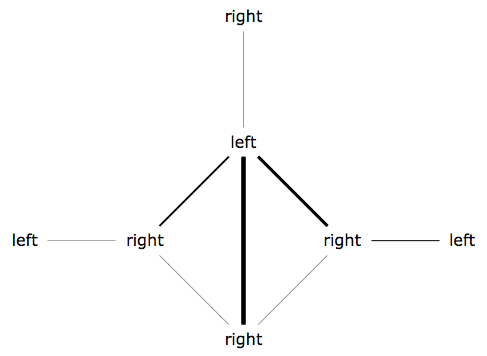
\includegraphics[width=8cm, height=6cm]{taking-sides-graph.png}\\
%  \caption{Grafo extraído de \cite{malouf-taking_sides}. Os vértices são usuários e as arestas, citações entre eles. Arestas mais escuras indicam frequência de citação mais alta.}
%  \label{fig:malouf}
%\end{figure}


%Padrões de citação a \emph{sites} também foram investigados \cite{efron}. No artigo de Miles Efron, os experimentos envolvem os \emph{datasets} \textbf{Political-Orientation} e \textbf{Artists}. O primeiro é composto de artigos políticos Estadunidenses de Direita ou Esquerda e o segundo é composto de textos sobre artistas musicais, divididos entre as categorias Alternativo e Popular. As taxas de acerto relatadas para as aplicações de Naïve Bayes nestes corpora foram de, respectivamente, 64.71\% e 50.1\%. A fim de melhorar as taxas de acerto na classificação dos documentos, o artigo estima a perspectiva de cada um deles avaliando a probabilidade de que eles sejam co-citados, na Web, com documentos referência de cada perspectiva. Estes documentos de referência são agrupados em listas de URLs. Esta metodologia, aplicada a \textbf{Political-Orientation}, resultou em uma taxa de acerto de 94.1\%. Para \textbf{Artists}, a taxa de acerto máxima obtida foi de 88.84\%.

%Todos os artigos que propuseram metodologias para melhorar a classificação em corpora com vocabulários muito uniformes consideraram algum esquema de citação. Se o corpus for composto de documentos pouco citados na Web, o esquema do artigo de Miles Efron pode não trazer nenhuma melhoria significativa ao problema. Se os autores dos documentos não mencionarem significativamente um ao outro, como aconteceu nos estudos com o \emph{dataset} \textbf{Politics}, a metodologia explorada por Tony Mullen e Robert Malouf não é recomendada. Essa área de pesquisa, portanto, ainda tem alguns problemas em aberto - e, considerando que estes três artigos foram escritos há mais de quatro anos, ela não parece atrair muita atenção. A justificativa para isso, provavelmente, tem a ver com o fato de que uniformidade no vocabulário não é um problema tão comum em Mineração de Perspectiva. No \textbf{capítulo X}, técnicas envolvendo comparação entre documentos, que podem trazer benefícios à classificação de \emph{datasets} difíceis - e neste caso também se enquadram aqueles em que o vocabulário é mais uniforme -, serão discutidas.

\section{Conclusões}
\label{freqs:conc}

%INTERNACIONALIZÁVEEEEEL!!
Este capítulo apresentou duas hipóteses linguísticas assumidas por métodos baseados em frequências de palavras: 1) palavras específicas, denominadas \emph{banner words}, costumam ser utilizadas para defender perspectivas diferentes e 2) a quantidade de vezes que uma palavra é mencionada em um documento está diretamente relacionada com seu enfoque \cite{teubert2001}. Como consequência, esses métodos funcionam melhor em \emph{datasets} nos quais o emprego de palavras varia significativamente por perspectiva. %tão melhor quanto mais diferentes forem os empregos de palavras por perspectiva.

%ideia de que pessoas costumam utilizar palavras específicas, denominadas \emph{stigma words} ou \emph{banner words}, para defender perspectivas diferentes. O uso de classificadores baseados na presença ou frequência das palavras, portanto, costuma funcionar bem na identificação dessas perspectivas. Entretanto, em alguns casos, as construções do discurso refletem diferentes perspectivas melhor do que o uso de palavras específicas. Nestes casos, as taxas de acerto desses classificadores são menores do que o desejado. 

Para ilustrar a relação entre as palavras de dois \emph{datasets} e o desempenho desses métodos, experimentos com o modelo de tópicos L-LDA foram executados. A extração das dez palavras mais fortemente associadas a cada tópico conduziu à visualização parcial de como o vocabulário dos \emph{datasets} se agrupa em torno de suas diferentes perspectivas. A informação, apesar de subjetiva, auxilia na compreensão das taxas de acerto obtidas com um classificador Naïve Bayes padrão, aplicado aos dois corpora. Para o primeiro \emph{dataset}, as taxas de acerto obtidas foram mais altas, o que pode ser explicado por uma presença maior de \emph{banner words} em comparação com o segundo \emph{dataset}.

Métodos baseados em frequências de palavras foram explorados pela maioria dos trabalhos revisados para esta monografia - mesmo fazendo parte de metodologias mais complexas. Apesar de outros fatores contribuírem para o mau desempenho destes métodos, como um número muito pequeno de documentos no \emph{dataset}, é interessante investigar o vocabulário do corpus caso as taxas de acerto obtidas estejam aquém do desejado. O uso de um modelo de tópicos L-LDA, agrupando palavras por perspectiva, é útil para compreender como os autores dos documentos se expressam. Se as palavras são empregadas de modo muito parecido por todas as perspectivas, isto justifica, ainda que em parte, o mau desempenho obtido.

% voa relação entre as palavras contidas em dois \emph{datasets} e suas diferentes perspectivas. No primeiro \emph{dataset}, as palavras extraídas para cada perspectiva se relacionam, semanticamente, melhor com a perspectiva em si do que no segundo \emph{dataset}. Neste último, palavras genéricas, como artigos e conjunções, se associam muito fortemente a todas as perspectivas, colaborando para uma uniformização do vocabulário. Isto explica, ainda que não seja trivial avaliar o quanto, as taxas de acerto mais altas obtidas com um Naïve Bayes no primeiro \emph{dataset}.

%Por fim, este capítulo também revisa artigos que discutem a questão do vocabulário do corpus. Estes artigos propõem metodologias para melhorar a classificação em \emph{datasets} cujo vocabulário é considerado muito uniforme - todas baseadas em algum esquema de citação a documentos. A questão do vocabulário do corpus é pouco discutida na literatura; provavelmente porque o problema é pouco comum e porque outros métodos, mais genéricos para \emph{datasets} difíceis de classificar, têm sido mais estudados.
 
%o primeiro \emph{dataset}, os artigos estão escritos sob uma das seguintes perspectivas: pró-Palestina ou pró-Israel. Por conta disso, o tópico \emph{pal} foi atribuído a todos os documentos pró-Palestina e o tópico \emph{isr}, a todos os pró-Israel. Estes tópicos facilitam a visualização das palavras mais fortemente associadas a cada uma das duas perspectivas, de acordo com o vocabulário empregado nos artigos. Um terceiro tópico, \emph{gen}, foi atribuído a todos os documentos, a fim de capturar as palavras que co-ocorrem neles independentemente de suas perspectivas. Após a execução do modelo, as 100 palavras mais fortemente associadas a cada um dos 3 tópicos foram coletadas. 35\% das associadas a \emph{isr} não estão presentes no conjunto recolhido para \emph{gen}. Para \emph{pal}, essa percentagem cai para 29\%. Por fim, 32\% das palavras mais fortemente associadas a \emph{isr} não fazem parte das 100 palavras mais fortemente associadas a \emph{pal} e vice-versa. Essas percentagens indicam que os autores dos documentos pró-Israel utilizam um vocabulário ligeiramente mais específico, na defesa de seus pontos de vista, do que os autores pró-Palestina. É importante ressaltar que nenhuma palavra foi filtrada na análise - ou seja, termos muito frequentes como \emph{the}, \emph{of} e \emph{and}, comumente extraídos dos \emph{datasets} antes da etapa de classificação, estavam presentes nos documentos processados pelo L-LDA.    

%Palavras associadas a \emph{isr} que não foram associadas a \emph{gen}
%['arafat', 'be', 'some', 'roadmap', 'us', 'yet', 'out', 'sharon', 'ariel', 'support', 'three', 'bush', 'palestine', 'new', 'terrorism', 'leader', 'then', 'jewish', 'after', 'arab', 'leadership', 'plan', 'president', 'than', 'bank', 'prime', 'regarding', 'like', 'could', 'violence', 'against', 'while', 'time', 'american', 'first']

%Palavras associadas a \emph{pal} que não foram associadas a \emph{gen}
%['then', 'some', 'authority', 'against', 'occupied', 'negotiations', 'occupation', 'sharon', 'united', 'end', 'way', 'palestine', 'international', 'be', 'after', 'plan', 'president', 'law', 'those', 'prime', 'land', 'i', 'violence', 'us', 'q', 'while', 'time', 'situation', 'first']

%Palavras associadas a \emph{pal} que não foram associadas a \emph{isr}
%['because', 'people', 'authority', 'states', 'right', 'occupied', 'any', 'negotiations', 'occupation', 'what', 'united', 'end', 'also', 'been', 'their', 'other', 'way', 'international', 'law', 'do', 'which', 'government', 'very', 'they', 'now', 'those', 'about', 'land', 'these', 'q', 'i', 'situation']

%Palavras associadas a \emph{isr} que não foram associadas a \emph{pal}
%['arafat', 'into', 'settlements', 'years', 'yet', 'out', 'even', 'would', 'ariel', 'west', 'support', 'three', 'bush', 'gaza', 'new', 'terrorism', 'leader', 'we', 'jewish', 'arab', 'most', 'leadership', 'minister', 'roadmap', 'than', 'bank', 'both', 'regarding', 'like', 'could', 'war', 'american']
%\textbf{As palavras estão ordenadas de acordo com a força da associação com cada um dos tópicos}


%\textbf{Lista de palavras e desempenho. Imagens e Tabelas.}

%Dado que em boa parte dos artigos estudados neste projeto, como \cite{lin-et-al2006} e \cite{klebanov}, atinge-se taxas de acerto superiores a 80\% com classificadores baseados em frequência de palavras, conclui-se que a mineração de perspectivas em discussões, artigos opinativos e debates requer metodologias diferentes, a depender de como as palavras foram escolhidas pelos autores dos documentos. %Nos debates estudados por \cite{hirst-et-al}, expressões de ataque e defesa são mais frequentes do que \emph{stigma words} e, como o método empregado no artigo foi um SVM treinado com frequências de palavras, observou-se que a classificação obtida para os lados do debate não refletia as perspectivas \emph{liberal} ou \emph{conservadora} - mas sim os lados \emph{oposição} (expressões de ataque) e \emph{situação} (expressões de defesa). 
%Estes estudos indicam a possibilidade de que, em debates e discussões nos quais há uma homogeneização do vocabulário empregado - o que pode acontecer quando todos os lados utilizam, em proporções similares, tanto expressões de ataque quanto de defesa -, classificadores baseados exclusivamente nas palavras utilizadas e/ou em suas frequências apresentarão má performance.

%A avaliação do desempenho desses classificadores\footnote{\textbf{SVMs e Naive Bayes padrão; LSPM}} nos \emph{datasets} estudados revela que artigos opinativos e notícias consolidaram perspectivas, através da escolha do vocabulário utilizado, melhor do que debates. Apesar disso, uma generalização neste sentido, restringindo o uso desses classificadores a artigos e notícias, não é recomendada por falta de indicativos linguísticos que comprovem essa tendência. Uma estratégia que pode ajudar na escolha ou descarte de um classificador desse tipo é uma análise das palavras que estão contidas nos documentos.

%\textbf{mostrar as percentagens prum dataset onde a linguagem eh mais uniforme. discutir.} 
%Explicar q isso nunca foi feito e q pessoas q ncontraram merda com essa feature fizeram outras coisas. descrever essas coisas.

%Estas hipóteses ilustram  
%Como indica \cite{}: 

%\textbf{MODO RASCUNHO AINDA}

%Explicar que uma diferença fundamental notada entre os datasets observados diz respeito à formalidade da linguagem empregada nos documentos. Enquanto alguns datasets utilizam documentos provenientes de meios onde a norma culta da linguagem impera, e uma revisão ortográfica é utilizada, outros são carregados de gírias, expressões e abreviações típicas da linguagem da Internet e contêm, eventualmente, grafias erradas para uma mesma palavra. <Dar exemplos textuais. Mostrar uma tabelinha, algo assim, indicando o volume de datasets com linguagem informal nos documentos estudados.> 

%A linguagem informal pode criar alguns desafios para a Mineração de Perspectiva [FECHAR O PROBLEMA EM: IDENTIFICAÇÃO DA PERSPECTIVA PRESENTE EM UM DOCUMENTO], especificamente no que diz respeito ao pré-processamento dos documentos e à escolha do método empregado. No pré-processamento, como indicado em (aaai-politics.pdf e 10.1.1.138.7160.pdf), a correção gramatical das palavras é bastante indicada. Com uma única versão de grafia para cada palavra (a correta), diminui-se a quantidade de ruído que grafias erradas podem causar na classificação.

%Uma característica dos datasets que deveria ser considerada sempre antes de se escolher o método utilizado - mas não é prática entre as pessoas que estudam perspective mining - é a frequência das palavras nos documentos do dataset. Se o léxico empregado pelos autores dos textos muda sensivelmente a depender de sua ideologia/perspectiva defendida/ponto de vista, é possível resolver o problema utilizando classificadores que usam essa frequencia como feature. GASTE TEMPO DANDO ALGUNS EXEMPLOS.  Em datasets informais, entretanto, como aponta Efron, a linguagem empregada por todos os lados da discussão pode ser basicamente a mesma: termos com forte carga de polaridade e gírias/jargões comuns na discussão [EXEMPLO]. Neste caso, é preciso utilizar métodos que utilizem mecanismos mais rebuscados do que a simples frequência/presença das palavras no texto. Alguns autores utilizam métodos mais gramaticais para lidar com datasets informais, como é o caso de , BLE e BLI. Os 2 primeiros criam o conceito de Opinion Frame (DEFINIR O CONCEITO). No primeiro caso, a ideia é associar corretamente opiniões a alvos, e associar alvos iguais utilizando técnicas de co-referência. Segundo Wiebe et al. (pegar a citação corretamente), ter as targets associadas, com as opiniões próximas, é uma boa forma de entender o overall de opiniões de um documento. A estratégia é uma alternativa possível para documentos em que as perspectivas estão muito associadas à linguagem opinativa, e onde essa linguagem é comum para todos os lados. Infelizmente, os resultados alcançados indicam que a tarefa não é trivial: blablablablababla (resolver coreferencia pra linkar targets não é tão simples assim => e dê exemplo). 

%uma diferença fundamental notada entre os \emph{datasets} observados diz respeito à formalidade da linguagem empregada nos documentos. Enquanto alguns datasets utilizam documentos provenientes de meios onde a norma culta da linguagem impera, e uma revisão ortográfica é utilizada, outros são carregados de gírias, expressões e abreviações típicas da linguagem da Internet e contêm, eventualmente, grafias erradas para uma mesma palavra. <Dar exemplos textuais. Mostrar uma tabelinha, algo assim, indicando o volume de datasets com linguagem informal nos documentos estudados.> 

\begin{table}[t]
\centering
\begin{tabular}{| p{10cm} | }
\hline

\emph{"The recent \textbf{Israeli} government decision to begin building extensive walls
around \textbf{Palestinian} is just one more example of how \textbf{Israeli} Prime
Minister Ariel Sharon is unable to deal with \textbf{Israeli} problems save
through his narrow security vision."} - Trecho extraído de artigo Pró-Palestina. \\ \hline

\emph{"The first conclusion that the Israeli political and security
establishment should learn and internalize after 18 months of
\textbf{Palestinian} Intifada, concerns the intensity of \textbf{Palestinian} blind
terrorism and guerilla warfare against the State of Israel."} - Trecho extraído de artigo Pró-Israel. \\ \hline

\end{tabular}
\label{3}
\caption{Trechos com as palavras \emph{palestinian} e \emph{israeli}, extraídos do \emph{dataset} \textbf{Bitterlemons}.}
\end{table}

\begin{table}[t]
\centering
\begin{tabular}{| p{10cm} | }
\hline

\emph{"\textbf{Bush}
and his advisers, who have been critical of Clinton's deep involvement
in a failed peace process ever since taking office, nevertheless
understood at the time that peace in the Middle East should be beyond
politics in America, and that the US could not permit itself to turn its
back on an Israeli leader who was determined to make peace."} - Trecho extraído de artigo Pró-Israel. \\ \hline

\end{tabular}
\label{4}
\caption{Trecho com a palavra \emph{bush}, extraído do \emph{dataset} \textbf{Bitterlemons}.}
\end{table}

\begin{table}[t]
\centering
\begin{tabular}{| p{10cm} | }
\hline
\emph{"But just as we were close to a complete
package that would have ended the \textbf{occupation} and established a
Palestinian state, Barak permitted Ariel Sharon's provocative visit to
Al Aqsa mosque, and launched his "revenge" on Palestinians."} - Trecho extraído de artigo Pró-Palestina. \\ \hline
\end{tabular}
\label{5}
\caption{Trecho com a palavra \emph{occupation}, extraído do \emph{dataset} \textbf{Bitterlemons}.}
\end{table}
% e  Termos associados ao Governo dos Estados Unidos, como \emph{bush} e \emph{american}, ilustram a relevância da aliança política estabelecida por Israel à época dos documentos. Palavras como \emph{occupation} e \emph{people}, por outro lado, ilustram a principal pauta Palestina no mesmo período: a ocupação da Faixa de Gaza.

%Os artigos deste primeiro \emph{dataset} foram escritos ou pelos editores do \emph{site} ou por convidados, divisão utilizada em \cite{lin-et-al2006} para avaliar o desempenho de um Naïve Bayes. No primeiro cenário, os documentos de treinamento eram os escritos pelos editores e os de teste, aqueles escritos pelos convidados; no segundo, tinha-se a situação inversa.

%As taxas de acerto obtidas com um classificador Naïve Bayes na identificação das perspectivas pró-Israel e pró-Palestina variaram entre 73.47\% e 98.98\%, a depender da divisão entre os conjuntos de treinamento e teste. %disponível em \cite{alibezz-nb}, as taxas de acerto obtidas foram de 73.47\% e 98.98\% para cada um dos cenários, respectivamente\footnote{A taxa de acerto obtida para o primeiro cenário foi significativamente inferior à obtida em \cite{lin-et-al2006} (85.85\%). Provavelmente, isto tem a ver com o número de iterações e as condições iniciais da execução.}. 

%O segundo \emph{dataset} estudado é o \textbf{Convote-Menor}, composto de colocações em debates da \emph{House of Representatives}, um dos dois órgãos principais do poder legislativo federal dos Estados Unidos. Os documentos foram marcados como sendo de parlamentares Republicanos ou Democratas, e como representando um posicionamento a favor ou contra a lei em pauta. Para este experimento, apenas a divisão entre Republicanos e Democratas foi considerada. O L-LDA foi aplicado a este \emph{dataset} de forma análoga ao primeiro experimento, e as dez palavras mais fortemente associadas a cada um dos tópicos - Genérico, Republicano e Democrata - estão listadas na Tabela 4.2. \emph{Stop words} também foram excluídas desta listagem.

%Ele é parte de um \emph{dataset} maior estudado pela primeira vez em \cite{thomas-pang-lee}, e está disponível em \cite{alibezz-convote}. A rotulação original dos documentos foi mantida neste \emph{dataset}: cada um deles é marcado com R, caso represente a colocação de um Republicano; ou D, no caso Democrata. Os documentos também são marcados com Y, caso representem a colocação de alguém que votou pela aprovação de uma lei; ou N, em caso contrário. Esta segunda marcação não foi explorada nesta monografia, nem a combinação das duas. O que se analisou, portanto, foi o desempenho do Naïve Bayes, disponível em \cite{alibezz-nb}, na classificação dos documentos como Republicanos ou Democratas.

%O L-LDA foi aplicado a este \emph{dataset} de forma análoga ao primeiro experimento, aproveitando os rótulos R e D, presentes nos documentos, como tópicos, e utilizando também um tópico genérico. As trinta palavras mais fortemente associadas a cada um dos tópicos, em ordem, podem ser conferidas na Tabela abaixo:

As listas de palavras da Tabela 4.2 indicam que o vocabulário do segundo \emph{dataset} não é suficiente para distinguir as perspectivas Republicana e Democrata. Parte das palavras, como \emph{bill}, \emph{legislation}, \emph{states} e \emph{act}, estão mais associadas ao processo legislativo \emph{per se} do que a alguma das perspectivas contidas nos documentos. A alta frequência de palavras como essas, empregadas pelos dois lados do debate, indica um cenário pouco polêmico, com menos \emph{banner words} e divergências. A palavra \emph{security}, por exemplo, fortemente associada às duas perspectivas, é utilizada de forma similar por ambas, como ilustrado na Tabela 4.6. Métodos baseados em frequências de palavras funcionam tão melhor quanto mais distintos forem os vocabulários empregados por cada perspectiva. Por este motivo, é esperado que suas taxas de acerto em \emph{datasets} como este não sejam altas.

\begin{table}[t]
\centering
\begin{tabular}{| p{10cm} | }
\hline

\emph{"Mr. speaker , I wholeheartedly agree that if we want to cut down on illegal immigration , we must improve border \textbf{security}. Just 2 weeks ago, an astute crane operator at the port of Los Angeles discovered 32 Chinese stowaways in a container that had just been unloaded from a Panamanian freighter."} - Trecho de discurso Democrata. \\ \hline


\emph{"The fence remains incomplete and is an opportunity for aliens to cross the border illegally. This incomplete fence allows border \textbf{security} gaps to remain open.  We must close these gaps because they remain a threat to our national \textbf{security}."} - Trecho de discurso Republicano. \\ \hline
\end{tabular}
\label{6}
\caption{Trechos com a palavra \emph{security}, extraídos do \emph{dataset} \textbf{Convote-Menor}.}
\end{table}


